\subsection{Kterm のメニュー}

Kterm のウィンドウ内で、
\KEYTOP{Ctrl} を押しながら \KEYTOP{ボタン 1} 〜 \KEYTOP{ボタン 3}
を押すことで、
 3 種類のメニューを出すことができる。

\begin{figure}[H]
\centering{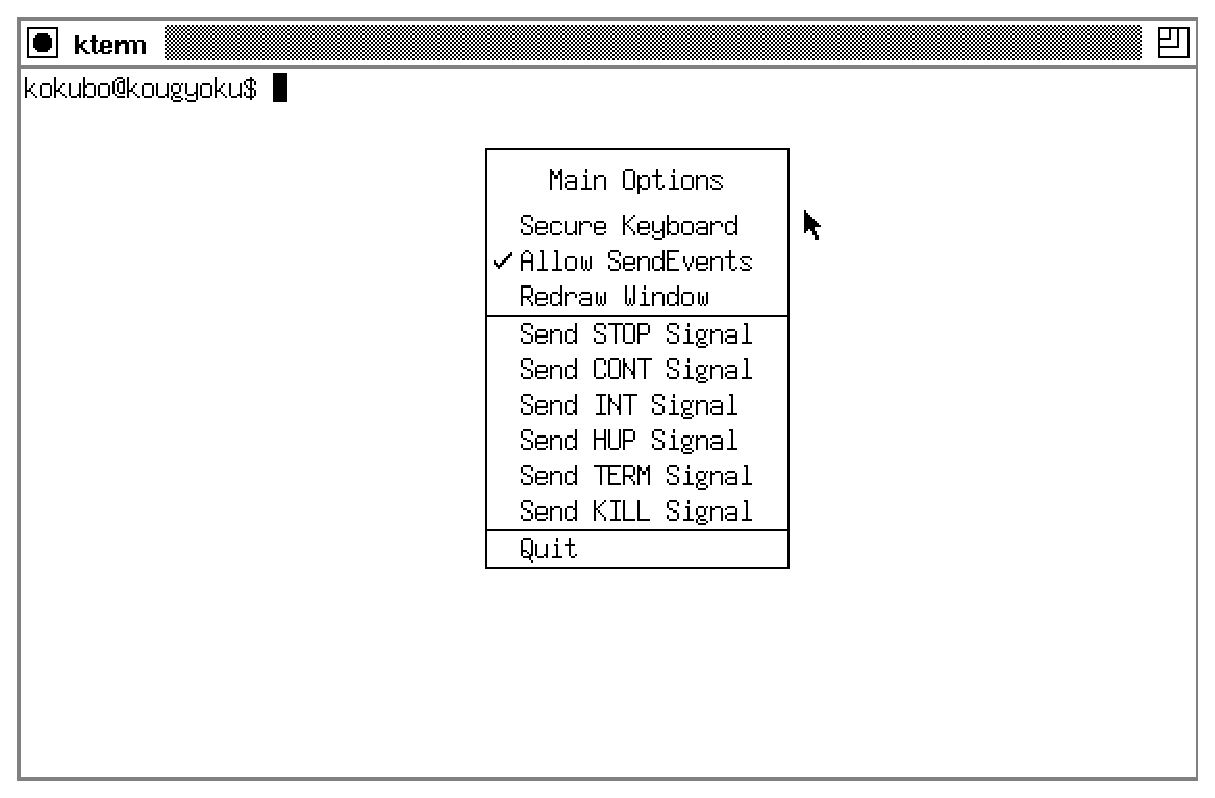
\includegraphics[scale=0.7]{ktermmenu.eps}}
\end{figure}

\begin{figure}[H]
\centering{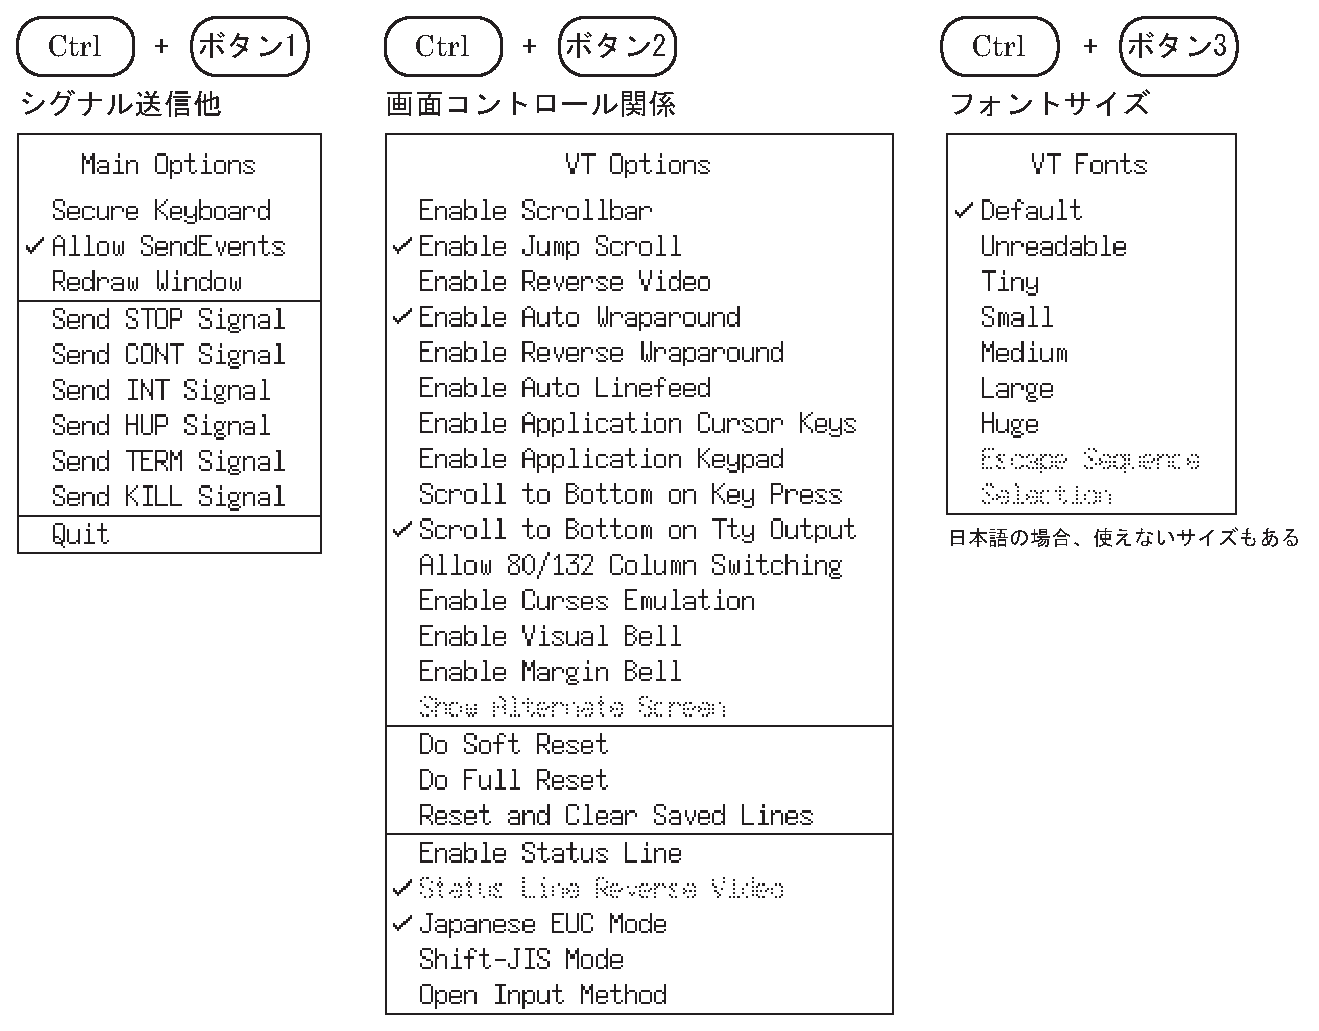
\includegraphics[scale=0.7]{ktermmenud.eps}}
\end{figure}

これらの内、 \KEYTOP{Ctrl}+\KEYTOP{ボタン 3} では、
フォントのサイズを変えることができる。
もしも、文字が小さく感じられるようであれば、
大きめに変更してみるといいだろう。
デフォルトは Tiny サイズである。
一部、日本語には対応していないサイズもあるので注意すること。

\subsubsection{スクロールバー}

Kterm を使っているときに使用頻度の高いスクロールバー
の使い方を紹介しよう。

まず、 Kterm のウィンドウ内で \KEYTOP{Ctrl}+\KEYTOP{ボタン 2}
で、メニューを出し、その一番上の
「Enable Scrollbar」を選ぶ。

\begin{figure}[H]
\centering{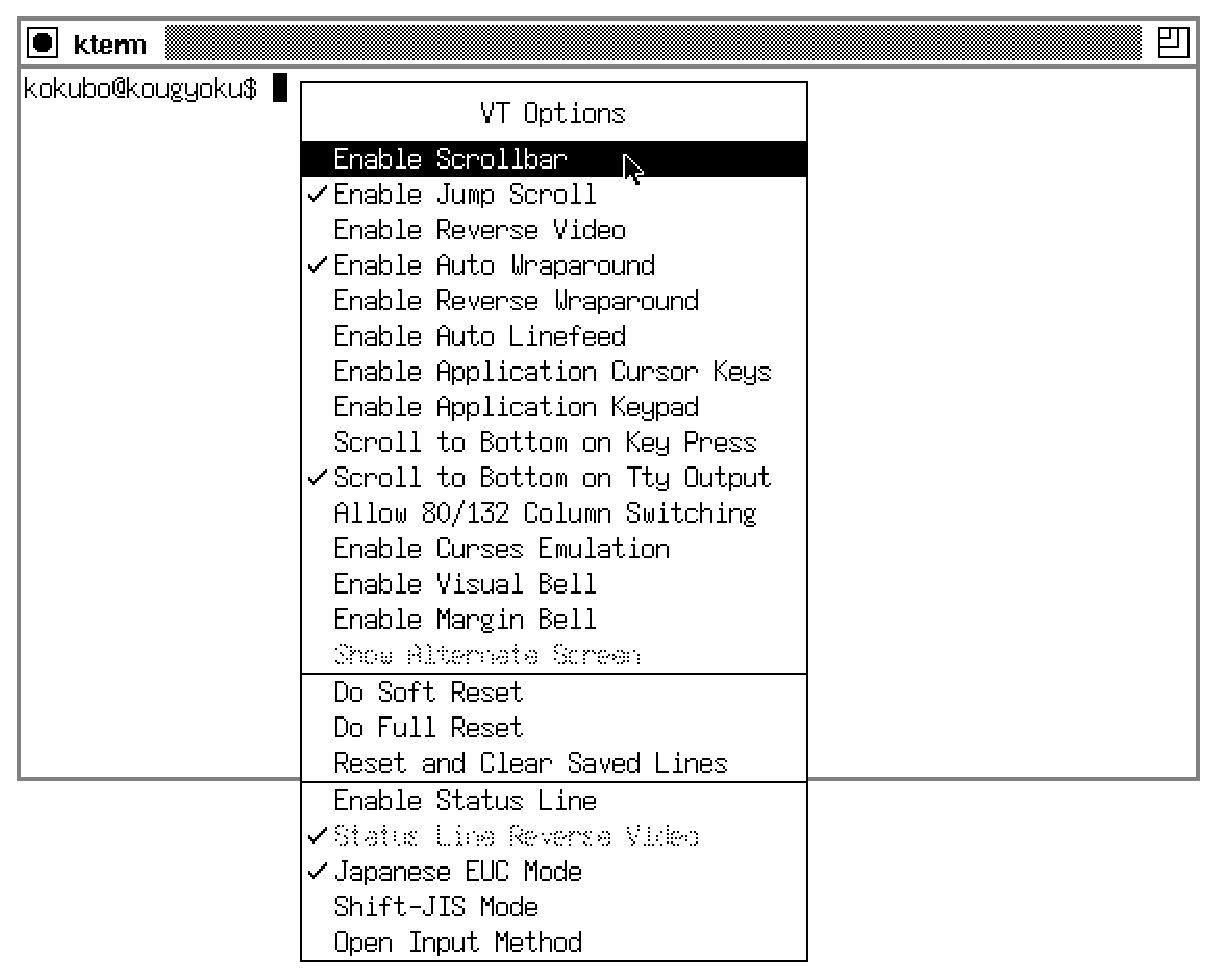
\includegraphics[scale=0.7]{enablescrollbar.eps}}
\end{figure}

すると、ウィンドウの左側にスクロールバーが現われる。

\begin{figure}[H]
\centering{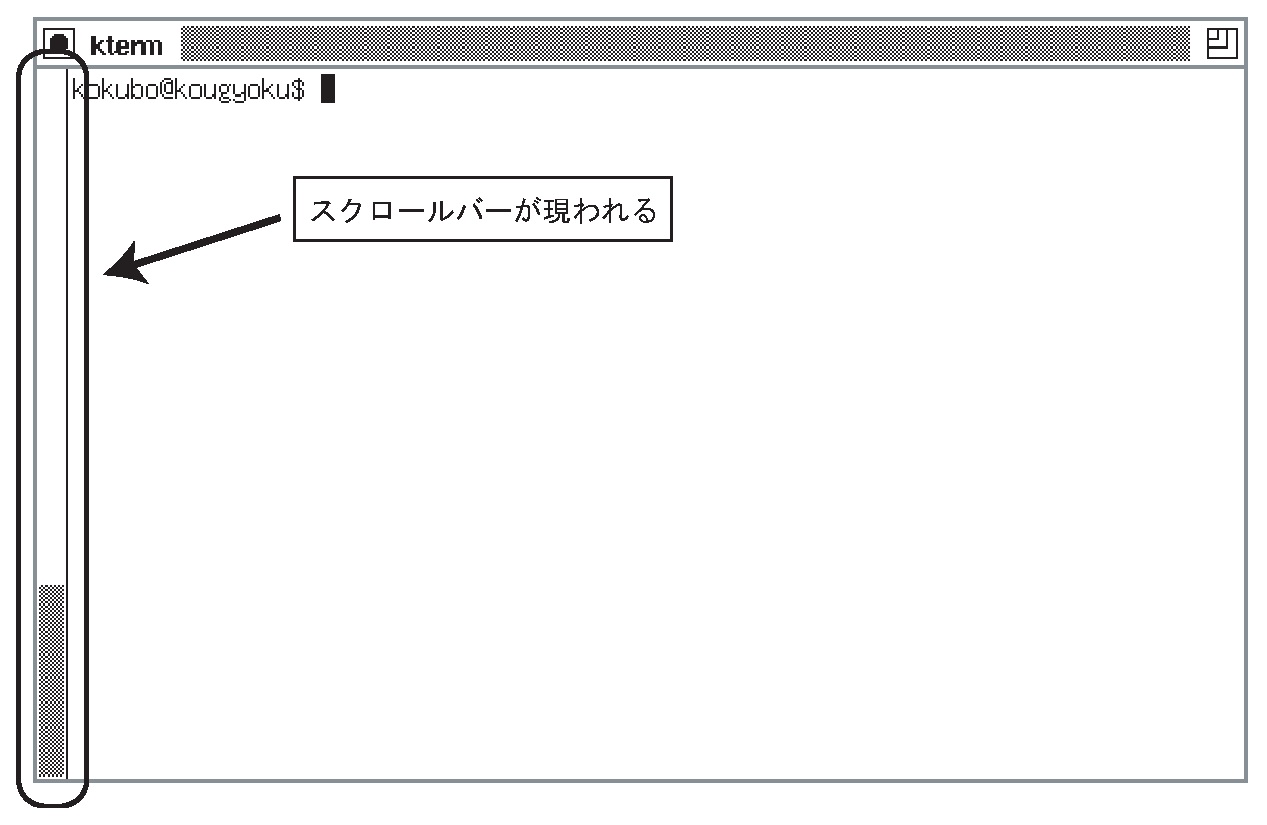
\includegraphics[scale=0.7]{scrollbar.eps}}
\end{figure}

2000 年のカレンダーを画面に表示するコマンド「\texttt{cal 2000}」
を打ってみる。

\begin{figure}[H]
\centering{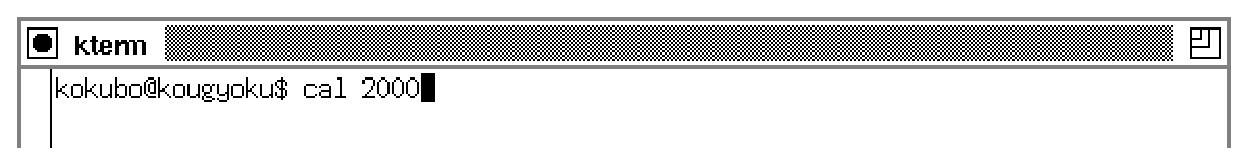
\includegraphics[scale=0.7]{cal2000.eps}}
\end{figure}

コマンドの出力結果が長すぎて、先頭の方が流れて読めなくなってしまう。

\begin{figure}[H]
\centering{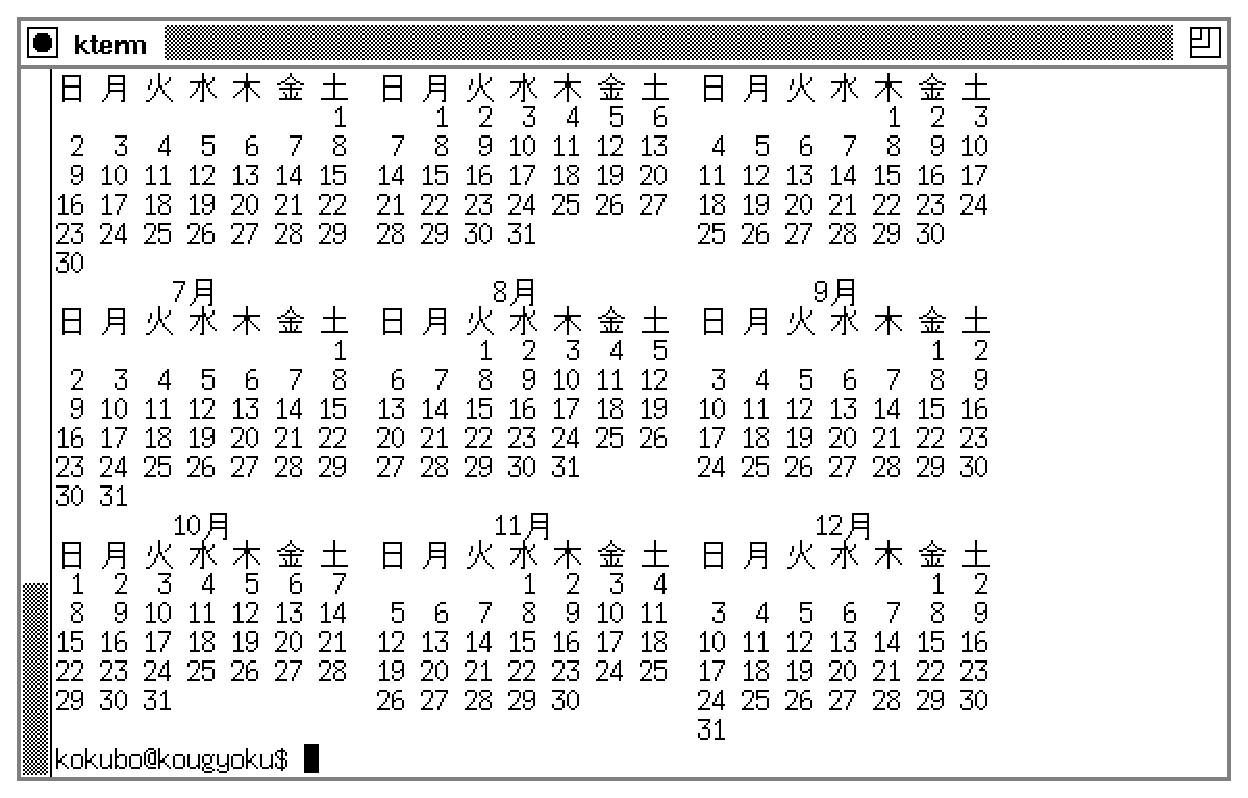
\includegraphics[scale=0.7]{fflow.eps}}
\end{figure}

マウス・カーソルをスクロールバーにのせると形が変わる。

\begin{figure}[H]
\centering{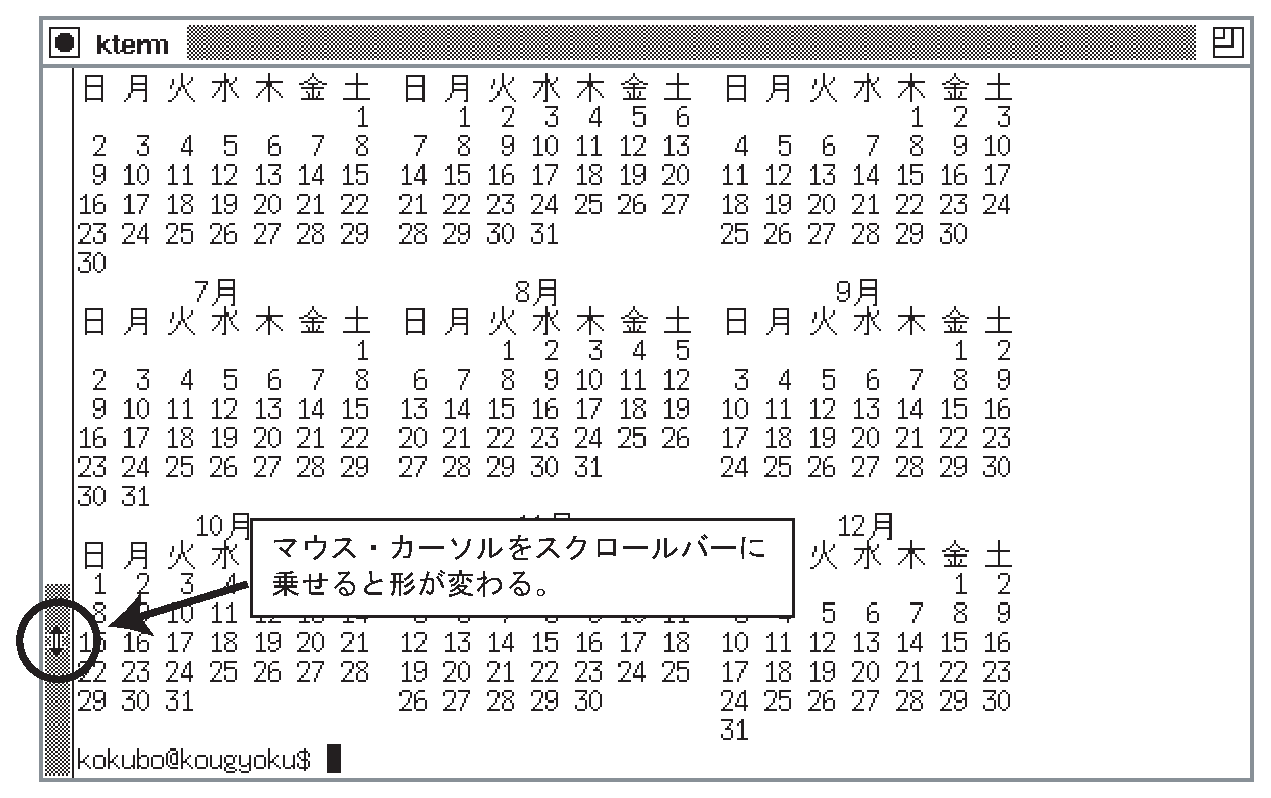
\includegraphics[scale=0.7]{scrollbarm.eps}}
\end{figure}

この状態で \KEYTOP{ボタン 2} を押したままドラッグすると、
画面が上下にスクロールして、前の部分も読むことができる。

\begin{figure}[H]
\centering{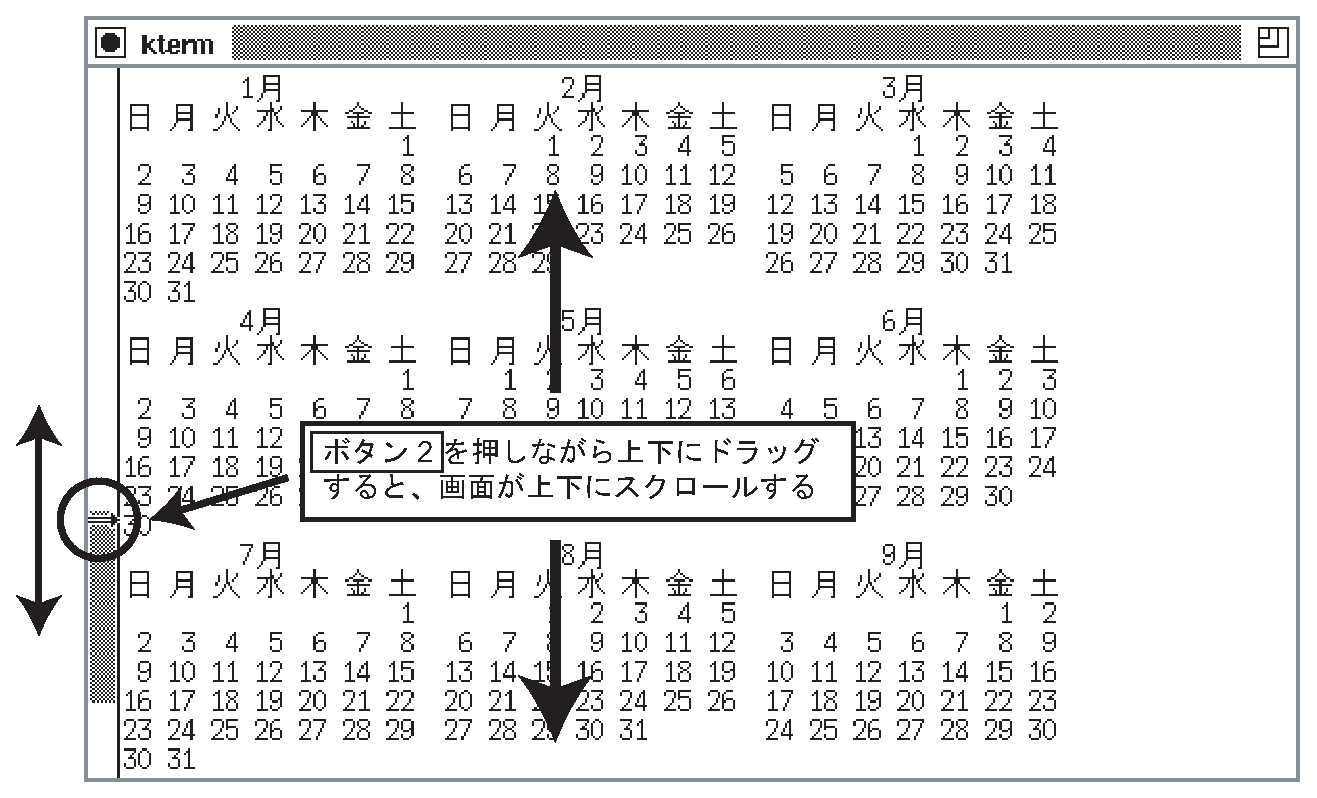
\includegraphics[scale=0.7]{scrolling.eps}}
\end{figure}
